% --- [ Back-end Components ] --------------------------------------------------

\subsection{Back-end Components}
\label{sec:design_back-end_components}

% TODO: Rewrite and clarify.

The back-end generates high-level control flow primitives such as if-statements and for-loops based on the structured CFG. In addition it translates the individual instructions of the LLVM IR to expressions and statements of the target programming language (in this case Go).

The back-end is responsible for translating the structured CFG of the LLVM IR into a target programming language. The \texttt{ll2go} tool is a proof of concept back-end which produces unpolished Go source code. The polishing is done by separate tools which fixes potential compilation issues and makes the code more idiomatic. The interaction between the middle-end and the back-end is illustrated in figure \ref{fig:back-end}. Currently the \texttt{go-post} replaces return-statements in the \texttt{main} function with calls to \texttt{os.Exit}, which is required since the \texttt{main} function has no return arguments in Go. Instead the Go runtime calls \texttt{os.Exit} with the status-code \texttt{0} once \texttt{main} returns to signal successful termination. This eliminates the need to always end the \texttt{main} function with a \texttt{return 0;} statement as is common practise in C. A future ambition is to make use of and possibly contribute to the \texttt{grind} tool which moves variable declarations closer to their usage, and thus improving readability of the code. Generally the aim is to keep the \texttt{ll2go} tool as simple as possible. The middle-end is responsible for the control flow analysis, and as a future ambition the data flow analysis. Since the complexity of the back-end is kept to a minimum it should be trivial to implement support for other output languages.

\begin{figure}[htbp]
	\begin{center}
		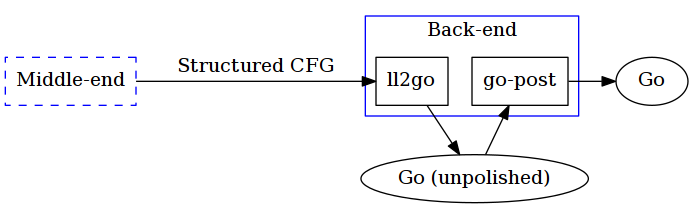
\includegraphics[width=\textwidth]{inc/back-end.png}
		\caption{foo}
		\label{fig:back-end}
	\end{center}
\end{figure}

% --- [ Subsubsections ] -------------------------------------------------------

% ~~~ [ Code Generation ] ~~~~~~~~~~~~~~~~~~~~~~~~~~~~~~~~~~~~~~~~~~~~~~~~~~~~~~

\subsubsection{Code Generation}
\label{sec:design_code_generation}

%    - Structured CFG -> Go ([ll2go](http://decomp.org/x/cmd/ll2go))
%       + Truthfully `ll2go` does not make direct use of `restructure` but rather the graph libraries.

foo

% Generates an abstract syntax tree (AST)

% ~~~ [ Post-processsing ] ~~~~~~~~~~~~~~~~~~~~~~~~~~~~~~~~~~~~~~~~~~~~~~~~~~~~~

\subsubsection{Post-processing}

%    - Unpolished Go -> Go ([go-post](http://decomp.org/x/cmd/go-post))

foo

The polishing is done by separate tools which fixes potential compilation issues and makes the code more idiomatic.

Currently the \texttt{go-post} replaces return-statements in the \texttt{main} function with calls to \texttt{os.Exit}, which is required since the \texttt{main} function has no return arguments in Go. Instead the Go runtime calls \texttt{os.Exit} with the status-code \texttt{0} once \texttt{main} returns to signal successful termination. This eliminates the need to always end the \texttt{main} function with a \texttt{return 0;} statement as is common practise in C. A future ambition is to make use of and possibly contribute to the \texttt{grind} tool which moves variable declarations closer to their usage, and thus improving readability of the code.

